\section{Login and Registration}

\begin{figure}[H]
	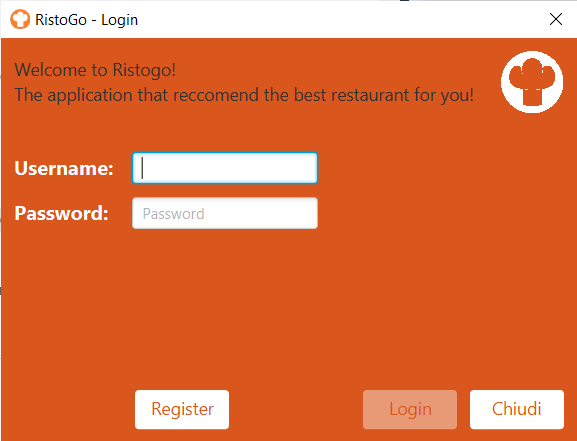
\includegraphics[width=\textwidth]{login}
	\caption{Login interface.}\label{fig:login}
\end{figure}

When the application starts it opens the main page (\figref{fig:login}), on
which an old user can insert username and password to login, clicking on the
button ``Login''.

Otherwise, if the user is a new one, he must do the registration procedure to
use the application.

If you want to close the application, click on the button ``Close''.

\subsection{Registration}

If you are a new user, click on ``Register'' on the main page to open the
registration form (\figref{fig:registration}).

Then, insert your username and your password (the password must contain at least
8 characters). Insert another time your password to confirm and then the city
where you lives If you went in the registration page wrongly, click on ``Login''
to return to the login page.

\begin{figure}[H]
	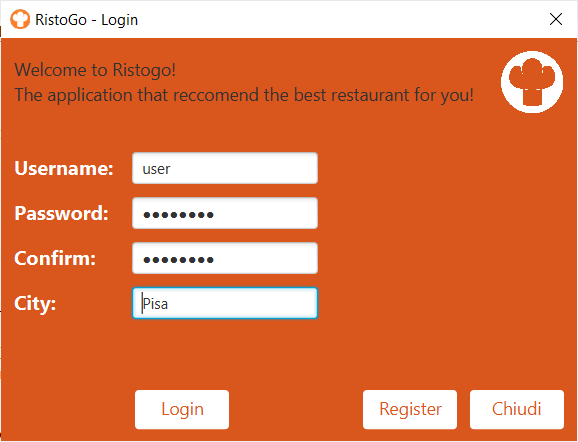
\includegraphics[width=\textwidth]{registration}
	\caption{Registration of a user.}\label{fig:registration}
\end{figure}

When you filled out the form, click on ``Register''. Now if you don’t receive
error messages your account will be create. So you can start to use the
application for the first time.
